 \let\negmedspace\undefined
\let\negthickspace\undefined
\documentclass[journal]{IEEEtran}
\usepackage[a5paper, margin=10mm, onecolumn]{geometry}
%\usepackage{lmodern} % Ensure lmodern is loaded for pdflatex
\usepackage{tfrupee} % Include tfrupee package

\setlength{\headheight}{1cm} % Set the height of the header box
\setlength{\headsep}{0mm}     % Set the distance between the header box and the top of the text

\usepackage{gvv-book}
\usepackage{gvv}
\usepackage{cite}
\usepackage{amsmath,amssymb,amsfonts,amsthm}
\usepackage{algorithmic}
\usepackage{graphicx}
\usepackage{textcomp}
\usepackage{xcolor}
\usepackage{txfonts}
\usepackage{listings}
\usepackage{enumitem}
\usepackage{mathtools}
\usepackage{gensymb}
\usepackage{comment}
\usepackage[breaklinks=true]{hyperref}
\usepackage{tkz-euclide} 
\usepackage{listings}
\def\inputGnumericTable{}                                 
\usepackage[latin1]{inputenc}                                
\usepackage{color}                                            
\usepackage{array}                                            
\usepackage{longtable}                                       
\usepackage{calc}                                             
\usepackage{multirow}                                         
\usepackage{hhline}                                           
\usepackage{ifthen}                                           
\usepackage{lscape}
\begin{document}

\bibliographystyle{IEEEtran}
\vspace{3cm}

\title{5.3.6}
\author{AI25BTECH11012 - GARIGE UNNATHI}
% \maketitle
% \newpage
% \bigskip
{\let\newpage\relax\maketitle}


\renewcommand{\thefigure}{\theenumi}
\renewcommand{\thetable}{\theenumi}
\setlength{\intextsep}{10pt} % Space between text and floats


\numberwithin{equation}{enumi}
\numberwithin{figure}{enumi}
\renewcommand{\thetable}{\theenumi}


\textbf{Question:}\\
If the pair of equations 3x - y + 8 = 0 and 6x - ry + 16 = 0 represents coincident
lines, then the value of r is  \\

\textbf{Solution:}\\
Let :
\begin{align}
    \vec{r_1} = \myvec{3 & -1 }\vec{x} = -8 \\
    \vec{r_2} = \myvec{6 & -r}\vec{x} = -16
\end{align}

For coincident lines:
\begin{align}
   Rank( \vec{r_1} \quad \vec{r_2})  = \myvec{3 & -1\\
                                              6 & -r}= 1
\end{align}

solving using above equation :
\begin{align}
   R_2 = R_2 - 2R_1\\
    =  \myvec{3 & -1\\
               0 & -r + 2}= 1
\end{align}

For the rank of above matrix to be one ,we need :

\begin{align}
   -r + 2 =0 \\
   r = 2 
\end{align}

\begin{figure}[h!]
   \centering
   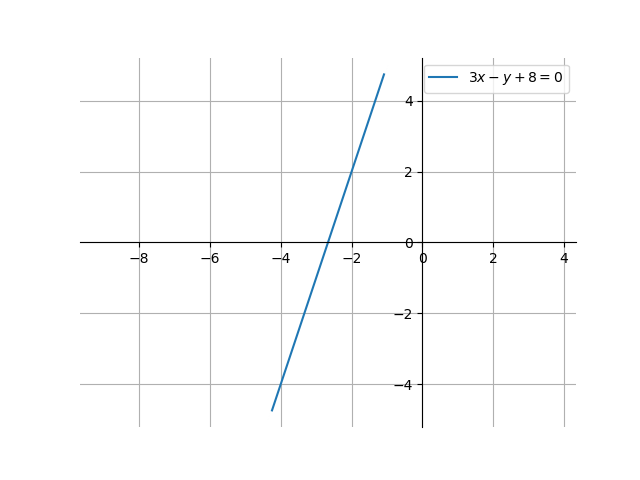
\includegraphics[width=0.7\linewidth]{/Users/unnathi/Documents/ee1030-2025/ai25btech11012/matgeo/5.3.6/figs/figs.png}
   \caption{}
   \label{stemplot}
\end{figure}








\end{document}
